\documentclass{article}

\usepackage{graphicx} % Required for inserting images
\usepackage{wrapfig}
\usepackage{amsmath} % For mathematical symbols and equations
\usepackage{natbib} % For citations   
\usepackage{floatflt}
\usepackage{amssymb}
\usepackage{booktabs}       % professional-quality tables
\usepackage{hyperref} % Web link
\usepackage{multicol} % Milti column

\newcommand\scalemath[2]{\scalebox{#1}{\mbox{\ensuremath{\displaystyle #2}}}}

\renewcommand{\arraystretch}{1.5}

\graphicspath{ {./images/} }

\title{LLaMAntino 3: Further Refinement of the Italian Language Using Consumer Hardware}
\author{Bruno Guzzo}
\date{Fall 2024}

\begin{document}
	
	\maketitle
	
	\begin{abstract}
		This project delves into the fine-tuning of a large language model (LLMs) for enhanced Italian language proficiency. 
		By employing 4-bit quantization, gradient checkpointing, and low-rank adaptation,we efficiently fine-tune the model on consumer hardware using a well-established Italian dataset.. 
		This method enables us to optimize the model's performance while minimizing computational overhead.
		To assess the impact of our fine-tuning strategy, we conduct a comprehensive evaluation using a series of Italian benchmarks, including those for question answering, commonsense reasoning, and natural language understanding.
		The project further explores the potential of incorporating a Retrieval-Augmented Generation (RAG) approach, based on a curated collection of Italian literature and novels.
	\end{abstract}
	
	\section{Introduction}
		Large Language Models (LLMs) have rapidly emerged as a transformative force in the field of artificial intelligence, demonstrating remarkable capabilities in understanding and generating human-like text. 
		These models, trained on massive datasets of text and code, leverage deep learning techniques to learn complex patterns and relationships within natural language. 
		At the core of their architecture lie several fundamental components:
		
		\begin{itemize}
			\item \textbf{Tokenization}: The process of breaking down text into smaller units, called tokens, which can be words, subwords, or even characters. This allows the model to process and represent the input text in a structured manner. 
			
			\item \textbf{Embedding}: Each token is then converted into a numerical vector, or embedding, which captures its semantic meaning in a high-dimensional space. This representation allows the model to understand relationships between words and their contextual significance.
			
			\item \textbf{Attention Mechanism}: This innovative mechanism, introduced in the seminal paper "Attention is All You Need" (Vaswani et al., 2017), enables the model to weigh the importance of different parts of the input sequence when processing information. This allows LLMs to effectively capture long-range dependencies and contextual nuances in text, a significant advancement over previous sequential models.
			
			\item \textbf{Transformers}: The dominant architecture for LLMs, transformers consist of multiple layers of self-attention and feed-forward neural networks. This structure allows for parallel processing of information, making them highly efficient and scalable for handling large datasets.
		\end{itemize}	
		
		The evolution of LLMs over the past decade has been marked by significant advancements in model size, training data, and architectural innovations. 
		Early models, such as recurrent neural networks (RNNs) and long short-term memory (LSTM) networks, faced limitations in capturing long-range dependencies and processing large amounts of data. 
		The introduction of the transformer architecture revolutionized the field, enabling the development of models with billions of parameters.
		These models have demonstrated impressive capabilities in various tasks, including text generation, translation, question answering, and code generation, sparking widespread interest and research in both academia and industry.
		
	\section{The Base Model: Meta LLaMA}
		
		\begin{figure}[h]
			\centering
			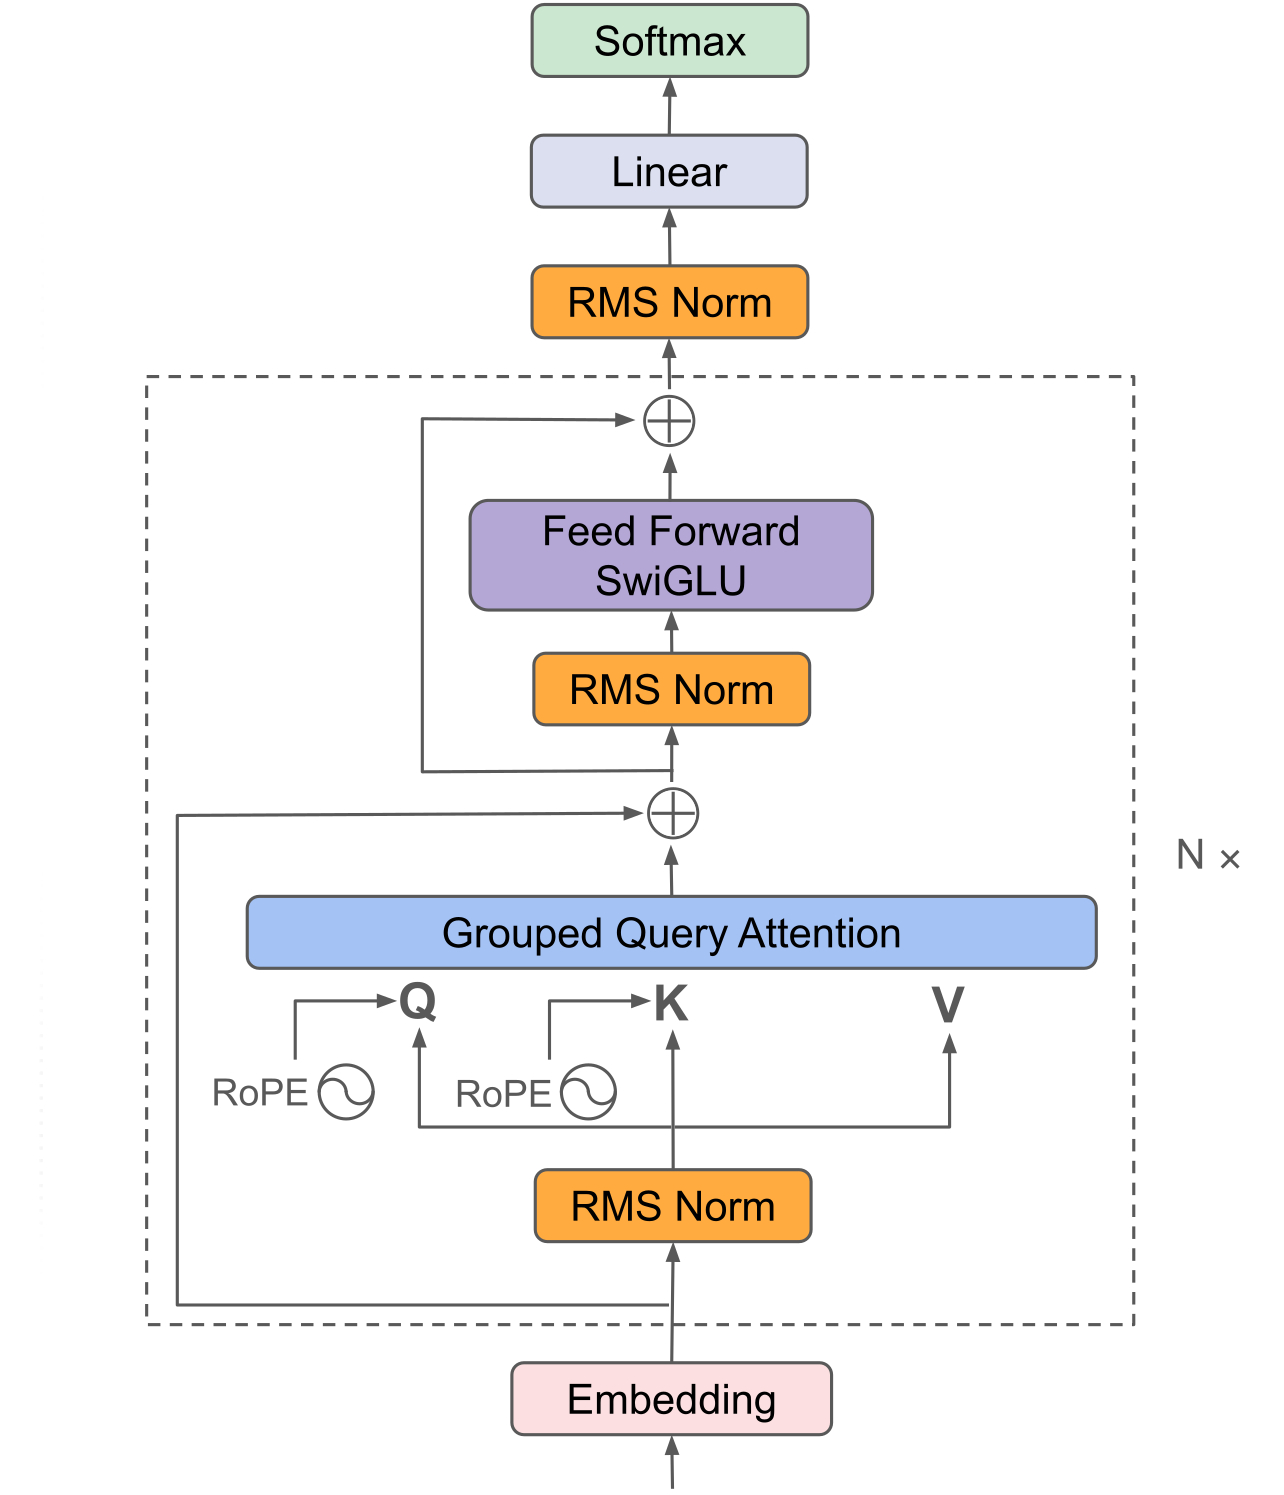
\includegraphics[width=6cm]{llama}
			\caption{LLaMA model architecture}
		\end{figure}
		
		The LLaMA models \cite{touvron2023llamaopenefficientfoundation} is a series of large language models (LLMs) ranging from 7B to 65B parameters, trained on trillions of tokens. 
		The goal of LLaMA is to achieve the best possible performance at various inference budgets.
		The model architecture is based on the transformer architecture, with the following modifications:
		
		\begin{itemize}
		
			\item 
				\textbf{Pre-normalization}: The input of each transformer sub-layer is normalized, rather than normalizing the output. The \textbf{RMSNorm} normalizing function \cite{zhang2019rootmeansquarelayer} is used. RMSNorm simplifies the LayerNorm (used by transfomer) by removing the re-centering operation, relying only on re-scaling. It normalizes the summed inputs to a neuron using the Root Mean Square (RMS) statistic.
				\begin{align}\label{eq_rmsnorm}
					\begin{split}
						& \bar{a}_i = \frac{a_i}{\text{RMS}(\mathbf{a})} g_i, \quad \text{where}~~ \text{RMS}(\mathbf{a}) = \sqrt{\frac{1}{n} \sum_{i=1}^{n} a_i^2}.
					\end{split}
				\end{align}
			
			\item
				\textbf{SwiGLU activation function}: The ReLU non-linearity is replaced with the SwiGLU (Swish-Gated Linear Unit) activation function. \\
				It is a combination of the \textbf{Swish activation function} and the \textbf{Gated Linear Unit} (GLU).
				
				\begin{align}\label{eq_swish_func}
					\begin{split}
						Swish(x) = x \cdot \sigma(x),  \quad GLU(x) = x \cdot \sigma(Wx + b)
					\end{split}
				\end{align}
				\begin{align}
					SwiGLU(x) = x \cdot \sigma(\beta \cdot x) + (1 - \sigma(\beta \cdot x)) \cdot (Wx + b)
				\end{align}
				
				Where \textbf{W}, \textbf{b} and $\boldsymbol{\beta}$  are trainable parameters. \\
				SwiGLU is \textbf{non-monotonic}, this allows it to capture complex non-linear relationships between input and output.
			
			\item 
				\textbf{Rotary Position Embeddings}: Absolute positional embeddings are removed, and instead rotary positional embeddings (RoPE)  \cite{su2023roformerenhancedtransformerrotary} are used at each layer of the network to compute query and key. \textbf{RoPE} is based on the idea of using a rotation matrix to control the inner product between query and value vectors.
				Let $x_m \in \mathbb{R}^d$ and $x_n \in \mathbb{R}^d$ be two word embeddings at positions $m$ and $n$, respectively. Let $q_m$ and $k_n$ be the corresponding query and key vectors. RoPE encodes the relative position information by rotating $q_m$ and $k_n$ by an angle that is proportional to $m-n$. The rotated vectors are then used to compute the inner product. Then, \textbf{the rotation matrix} is defined as follows: 
				\begin{equation}
					\scalemath{0.75}{
						R^d_{\Theta,m} = 
						\begin{pmatrix}
							\cos{m\theta_1}& -\sin{m\theta_1}&0&0&\cdots&0&0\\
							\sin{m\theta_1}&\cos{m\theta_1}&0&0&\cdots&0&0 \\
							0&0&\cos{m\theta_2}& -\sin{m\theta_2}&\cdots&0&0\\
							0&0&\sin{m\theta_2}&\cos{m\theta_2}&\cdots&0&0 \\
							\vdots&\vdots&\vdots&\vdots&\ddots&\vdots&\vdots\\
							0&0&0&0&\cdots&\cos{m\theta_{d/2}}& -\sin{m\theta_{d/2}}\\
							0&0&0&0&\cdots&\sin{m\theta_{d/2}}&\cos{m\theta_{d/2}}
						\end{pmatrix}
					}
					\label{fn:rope-RMat}
				\end{equation}
				Where $\Theta = \{\theta_i = 10000^{-2(i-1)/d}, i \in [1, 2, ..., d/2]\}$ is a set of pre-defined parameters.
				The inner product of the rotated vectors is then computed as follows:
				\begin{equation}
					q_m^T k_n = (R_{\Theta,m}^{d} W_q x_m)^T (R_{\Theta,n}^{d} W_k x_n) = x_m^T W_q R_{\Theta,n-m}^{d} W_k x_n
					\label{q_k_inner_product}
				\end{equation}
				Where $R_{\Theta,n-m}^{d} = (R_{\Theta,m}^{d})^T R_{\Theta,n}^{d}$. \\
				This inner product decays with increasing relative distance $|m - n|$. This is due to the rotation matrix $R_{\Theta,n-m}^{d}$ becoming more diagonal and thus decreasing the overall cosine value of the angel between $q$ and $k$ vectors.
				
				
		\end{itemize}
		
		\begin{table*}[h]
			\center
			\begin{tabular}{ccccccc}
				\toprule
				params & dimension & $n$ heads & $n$ layers & learning rate & batch size & $n$ tokens \\
				\midrule
				6.7B  & 4096 & 32 & 32 & $3.0e^{-4}$ & 4M & 1.0T \\
				13.0B & 5120 & 40 & 40 & $3.0e^{-4}$ & 4M & 1.0T \\
				32.5B & 6656 & 52 & 60 & $1.5e^{-4}$ & 4M & 1.4T \\
				65.2B & 8192 & 64 & 80 & $1.5e^{-4}$ & 4M & 1.4T \\
				\bottomrule
			\end{tabular}
			\caption{\textbf{LLaMA Model sizes, architectures, and optimization hyper-parameters}}
		\end{table*}  
		
	\section{LLaMA 3}	
		LLaMA \cite{dubey2024llama3herdmodels} 3 is a series of large language models (LLMs) developed by Meta AI. It is the successor to the LLaMA model, featuring significant enhancements in terms of scale, performance, and capabilities. A key improvement from LLaMA to LLaMA 3 is the adoption of the \textbf{Grouped Query Attention} (GQA). It is a type of attention mechanism that groups the queries into a smaller number of groups where each group shares a single key and value. This strategy reduces the number of attention weights that need to be computed leading to faster training and computation.
		
	
		\begin{table*}[h]
			\center
			\begin{tabular}{ |p{4cm}|p{4cm}|p{4cm}| }
				\hline
				\textbf{Feature} & \textbf{LLaMA} & \textbf{LLaMA 3} \\
				\hline
				\textit{Normalization} & RMSNorm (before self-attention) & RMSNorm (before self-attention) \\
				\hline
				\textit{Activation Function} & SwiGLU & SwiGLU \\
				\hline
				\textit{Positional Embedding} & RoPE & RoPE \\
				\hline
				\textit{Attention} & Standard Multi-Head Attention & Grouped Query Attention (GQA) \\
				\hline
				\textit{Attention Mask} & No attention mask & Attention mask to prevent self-attention between different documents in the same sequence \\
				\hline
				\textit{Tokenizer} & SentencePiece Byte Pair Encoding (BPE) & SentencePiece BPE with Tiktoken vocabulary \\
				\hline
				\textit{Vocabulary Size} & 32,000 tokens & 128,000 tokens \\
				\hline
				\textit{Context Window} & 2048 tokens & 128K tokens \\
				\hline
			\end{tabular}
			\caption{\textbf{LLaMA 3 and LLaMA key differences}}
		\end{table*}  
	
		LLAMA 3 undergoes a post-training process that aligns it with human feedback.
		This process involves \textbf{Supervised Fine-Tuning} (SFT) and \textbf{Direct Preference Optimization} (DPO). SFT is conducted on a mixture of human-annotated and synthetically-generated data, while DPO utilizes human-annotated preference data.
		
	\section{LLaMAntino 3 8B}
	\textbf{LLaMAntino 3 8B} 'ANITA' \cite{polignano2024advanced} is Italian language LLM based on the Meta's LLaMA 3 8 billion parameters model. It is developed and maintained by the \textbf{SWAP Team} of the Bari University, Italy. It is fine-tuned using a combination of \textbf{Supervised Fine-Tuning} (SFT) and \textbf{Dynamic Preference Optimization} (DPO) to achieve superior performance in the Italian language. \\
	The fine-tuning process involved two main steps: 
	
	\begin{itemize}
		\item 
			\textbf{Model Supervised Fine-Tuning}: The starting point is the \textbf{meta-llama/Meta-Llama-3-8B-Instruct} model, an instruction tuned version of the base LLaMa 3 8B model. 
			Then, it has been fine-tuned using a dataset named \textbf{Chat-Error/wizard\_alpaca\_dolly\_orca}, this dataset is a combination of three well-known datasets: WizardLM\_Orca, Dolly-v2\_Orca, and Alpaca\_Orca. 
			It consists of 100K prompts organized into system, instruction, input, and output fields in English language.	The model was fine-tuned using the \textbf{Unsloth framework} on an NVIDIA H100 64GB GPU card.
		
		\item 
			\textbf{Model Direct Preferences Optimization}: After SFT, DPO was applied to align the model's outputs with human preferences. For this purpose, the \textbf{mlabonne/orpo-dpo-mix-40k} dataset has been used, which contains approximately 40k examples from various sources like \textbf{Capybara-Preferences}, \textbf{distilabel-intel-orca-dpo-pairs}, and \textbf{ultrafeedback\\-binarized-preferences-cleaned}.
			The DPO process was also conducted using Unsloth on an NVIDIA H100 64GB GPU card.
	\end{itemize}
	
	To adapt the model to the Italian language, we used the \textbf{gsarti/clean\_mc4\_it} dataset, which is a cleaned version Italian split of the multilingual colossal Common Crawl's \textbf{Web Crawl Corpus} (mC4).
	This dataset has been used with the same SFT strategy as before, formatting the prompts according to the standard LLaMA 3 template. \\
	Then, the model has been evaluated using several benchmarks, including \textbf{MMLU}, \textbf{HellaSwag},\textbf{ A12 Reasoning Challenge} (arc\_c), TruthfulQA, Winogrande, and GSM8K. 
	The results showed outstanding performance compared to similar and larger models, demonstrating the effectiveness of our fine-tuning strategy.
	
	\begin{table*}[h]
		\center
		\begin{tabular}{cc}
			\toprule
			\textbf{Metric} & \textbf{Value} \\
			\midrule
			Avg. & 0.6160 \\
			Arc\_IT & 0.5714 \\
			Hellaswag\_IT &	0.7093 \\
			MMLU\_IT & 0.5672 \\
			\bottomrule
		\end{tabular}
		\caption{\textbf{LLaMAntino 3 'ANITA' Main Benchmark Result}}
	\end{table*}  

	\section{Optimizations}
	Prior to running fine-tuning experiments on LLaMAntino 3 model various optimization strategy is needed. This strategies ensure that the model can run and train on a consumer based hardware without causing out of memory errors or being too slow. 
	The optimization strategy used is the following.
	
	\subsection{Quantization}  
	Large neural networks, are computationally expensive and memory-intensive. This makes them difficult to deploy on resource-constrained devices. Quantization addresses this by reducing the numerical precision of the network's weights and activations, typically from 32-bit floating-point to lower bit-depth representations like 8-bit or 4-bit integers. The core idea behind quantization is to map the range of real-valued weights and activations to a smaller set of quantized values. A common approach is to use an affine mapping:
	\begin{equation}
		r=S(q-Z)
	\end{equation}
	Where \textbf{r} is the real value, \textbf{q} is the quantized value, \textbf{S} is the scale factor and \textbf{Z} is the zero-point. To minimize accuracy loss, quantized training simulates the effects of quantization during the training process. This allows the network to adapt to the lower precision representation. During training, weights and activations are quantized in the forward pass, but gradients are still computed and updated in floating-point.
	
	
	\subsection{Low Rank Adaptation (LoRA)}
	The core idea of Low-Rank Adaptation (LoRA) \cite{hu2021loralowrankadaptationlarge} is rooted in the observation that the changes in a model's weights during adaptation to a new task often exhibit a low rank.
	This means that the updates to the weight matrices can effectively be represented by a much smaller set of basis vectors. LoRA leverages this property to significantly reduce the number of trainable parameters during adaptation. \\
	Consider a \textbf{pre-trained weight matrix} $W \in \mathbb{R}^{d \times k}$ within a neural network layer, such as a fully connected layer or an attention head in a Transformer model. During adaptation, this weight matrix is typically updated through gradient descent, resulting in a change $\Delta W$. LoRA posits that $\Delta W$ can be approximated by a \textbf{low-rank decomposition}:
	\begin{equation}
		\Delta W \approx B A
	\end{equation}
	Where $A \in \mathbb{R}^{r \times k}$ and $B \in \mathbb{R}^{d \times r}$ are matrices with $r \ll \min(d, k)$. Here, $r$ represents the \textbf{rank of the decomposition}, which is assumed to be much smaller than the original dimensions of the weight matrix.
	The forward pass through the layer is then modified to incorporate the low-rank update:
	\begin{equation}
	h = W x + B A x = (W + B A) x
	\end{equation}
	Where $x$ is the input to the layer and $h$ is the output and $\Delta W x$ is also scaled by $\frac{\alpha}{r}$, where $\alpha$ is a constant in $r$. \\
	During training, \textbf{the original weight matrix $W$ is frozen}, and only the matrices $A$ and $B$ are updated. Both $A$ and $B$ are initialized using a random Gaussian distribution.
	By training only the low-rank matrices, the number of trainable parameters is significantly reduced, leading to \textbf{substantial memory savings}.
	
	\subsection{Gradient Checkpointing}  
	Gradient checkpointing is a technique used to reduce the memory consumption of deep neural network training. 
	It is based on the idea that instead of storing all intermediate activations of a neural network during the forward pass, only a subset of these activations need to be stored.
	The remaining activations can be recomputed during the backward pass, thereby trading off computation time for memory savings.
	Let's consider a neural network with $n$ layers. We can denote the activations of the network at layer $i$ as $a_i$. The forward pass of the network can be written as:
	\begin{equation}
		a_i = f_i(a_{i-1}, w_i)
	\end{equation}
	Where $f_i$ is the function computed by layer $i$ and $w_i$ are the weights of layer $i$.
	The backward pass of the network can be written as:
	\begin{equation}
	\frac{\partial L}{\partial a_{i-1}} = \frac{\partial L}{\partial a_i} \frac{\partial a_i}{\partial a_{i-1}}
	\end{equation}
	Where $L$ is the loss function. To compute the gradients of the loss function with respect to the activations, we need to store all the activations $a_i$ during the forward pass. This can be \textbf{memory-intensive}, especially for deep neural networks.
	Gradient checkpointing addresses this issue by only storing a subset of the activations, called checkpoints. 
	Let's denote the checkpoints as $c_k$, where $k$ is the index of the checkpoint. The forward pass of the network with gradient checkpointing can be written as:
	\begin{gather}
		a_i = f_i(a_{i-1}, w_i) \text{ if $i$ is not a checkpoint} \\
		c_k = a_i \text{ if $i$ is a checkpoint}
	\end{gather}
	During the backward pass, the activations that are not checkpoints are recomputed from the nearest checkpoint ($a_i = f_i(a_{i-1}, w_i)$). The backward pass with gradient checkpointing can be written as:
	\begin{gather}
		\frac{\partial L}{\partial a_{i-1}} = \frac{\partial L}{\partial a_i} \frac{\partial a_i}{\partial a_{i-1}} \text{ if $i$ is not a checkpoint} \\
		\frac{\partial L}{\partial c_k} = \frac{\partial L}{\partial a_i} \frac{\partial a_i}{\partial c_k} \text{ if $i$ is a checkpoint}
	\end{gather}
	
	\section{LLaMAntino 3 8B: Further Fine-Tuning}
	The objective of this project is to test whether it is possible to further extend the capabilities of the LLaMAntino 3 model to generalize and handle Italian language tasks, such as chatting.
	Since the adoption of the optimization strategy discussed above has proved necessary to run this kind of model locally, we run some of the same benchmarks proposed by the authors to check how these optimizations impact the overall model performance. 
	A description of those benchmarks is present in the appendix section.  
	To save time, we chose to adopt a 0.20\% subset of the proposed datasets used by the authors for the chosen benchmarks.
	
	\begin{table*}[h]
		\center
		\begin{tabular}{ccc}
			\toprule
			\textbf{Metric} & \textbf{Original Value} & \textbf{Our Value} \\
			\midrule
			Arc\_IT & 0.5714 & 0.5256 \\
			Hellaswag\_IT &	0.7093 & 0.6775 \\
			\bottomrule
		\end{tabular}
		\caption{\textbf{LLaMAntino 3, 4-bit Quantization, 20\% Dataset}}
	\end{table*}
	
	\subsection{Italian Wikipedia Dataset}
	The first way we chose to try to extend the model generalization capability and enhance its knowledge regarding the Italian language is to fine-tune the model on the whole Italian Wikipedia dataset, available online.
	This first idea is justified since part of this dataset and its variants have been commonly used in the training of successful LLMs like OpenAI's GPT family. The dataset we chose has roughly 1.83M rows with fields such as title, text, and URL. More details can be found \href{https://huggingface.co/datasets/wikimedia/wikipedia/viewer/20231101.it}{here}.
	
	\subsubsection{Fine-Tuning process}
	The fine-tuning was made possible by the adoption of the optimizations described above, and the overall fine-tuning for one epoch took roughly 50 hours on an 8GB GPU.
	We chose a LoRA rank ($r$) equal to 32. This allowed us to train roughly 83M parameters, i.e., 8.3\% of the total model parameters.
	If we take into account the hardware used, though this number may not appear significant, it is still a huge result comparing the consumer hardware we used and the enterprise hardware used to build and train the original model.
		
	\subsubsection{Perplexity Score}
	\textbf{Perplexity} is a metric used to assess the performance of a language model (LM).	It measures how well the model predicts a sequence of tokens (e.g., words) by quantifying the uncertainty or "surprise" the model exhibits when encountering the sequence. Formally, given a sequence of tokens $X=(x_1,x_2,...,x_n)$, the perplexity (PP) of the language model on this sequence is calculated as:
	\begin{equation}
		\text{PPL}(X) = \text{exp}(-\frac{1}{N} \sum_{i=1}^{N} \log_2 P(x_i | x_{1:i-1}))
	\end{equation}
	Where: $P(x_i | x_{1:i-1})$ is the probability assigned by the model to the token $x_i$ given the preceding tokens $x_1,...,x_{i-1}$. In essence, perplexity is the exponentiated average negative log-likelihood of the sequence. A lower perplexity score indicates better performance, as it implies that the model assigns higher probabilities to the observed tokens, thus exhibiting less surprise.\\
	To measure how the fine-tuning process has impacted the LLaMAntino 3 model we computed the perplexity score over a 0,01\% random sample of the Italian Wikipedia dataset. This is done to reduce the computational cost and correspond to extracting roughly 18k rows from the dataset.
	We used a sliding window approach to process the tokenized text in smaller chunks. This is necessary because language models have limitations on the length of input sequences they can handle. Nevertheless, the size of input sequences directly affects memory consumption.
	We choose a size of \textbf{64} for both the step size for the sliding window (stride) and the maximum length of each input sequence. This means there is no overlap between windows.
	
	\begin{table*}[h]
		\center
		\begin{tabular}{ccc}
			\toprule
			\textbf{LLaMA 3 8B} & \textbf{LLaMAntino 3 8B} & \textbf{Our Model} \\
			\midrule
			15.923903 & 18.758045 & 11.394022 \\
			\bottomrule
		\end{tabular}
		\caption{\textbf{PPL measure on random under-sampled Wikipedia IT}}
	\end{table*} 

	The result shows how the performance of our fine-tuned model is superior to those obtained from both LLaMAntino 3 and LLAMA 3. It is worth noting that LLAMA 3 shows superior performance over LLaMAntino 3. Our hypothesis is that due to the extensive LLaMAntino 3 fine-tuning in different contexts, it has been biased toward a different language style and behavior.  
	
	\subsubsection{Common Benchmarks Scores}
	\begin{table*}[h]
		\center
		\begin{tabular}{ccc}
			\toprule
			\textbf{Metric} & \textbf{Original Value} & \textbf{Our Value} \\
			\midrule
			Arc\_IT & 0.5256 & 0.4188 \\
			Hellaswag\_IT &	0.6775 & 0.5182 \\
			\bottomrule
		\end{tabular}
		\caption{\textbf{LLaMAntino 3, Full Wikipedia IT, $r=32$, $\alpha=8$}}
	\end{table*} 
	
	Despite the resources employed, there has been a significant decrease in the chosen benchmark metrics. Our hypothesis is that the information and text in the Wikipedia IT dataset is not well suited for the benchmark chosen by the authors. However, we expected that the model performance would not degrade, at least for the ARC benchmark, which is based on grade-school-level, multiple-choice science questions.
	
	\subsection{Empirical results}
	To gain a glimpse of how this fine-tuning has changed the model, we propose a set of prompts given to both non-tuned and tuned models. We have then preserved the same value of \textbf{top-p}=0.95 and \textbf{temperature}=0.6 along with a maximum output size of 256 tokens. \\
	
	\textbf{Wikipedia IT Fine-Tuned Model}:
	\begin{enumerate}

		\item 
		\textbf{Prompt}: Scrivi una breve storia per bambini in rima sulla vita di Leonardo da Vinci, usando un linguaggio semplice e fantasioso.\\
		\textbf{Response}: \textit{Leonardo da Vinci nacque a Vinci, in Toscana, in una famiglia numerosa di artisti. Il padre fu un pittore e la madre una modella.\\\\Quando Leonardo era bambino, suo padre lo portò a Firenze, dove il piccolo si appassionò alla pittura, ai disegni e alle sculture. Il padre lo fece studiare pittura con un pittore locale, ma Leonardo preferì andare a Milano per studiare scultura con il famoso pittore Andrea del Verrocchio. Il maestro lo aiutò a diventare un ottimo scultore.\\\\Ma Leonardo aveva anche un grande interesse per le macchine, le invenzioni e le scoperte scientifiche. In seguito si dedicò a molti altri interessi: architettura, musica, matematica, ingegneria, letteratura e medicina. Inoltre, fu un pioniere dell'aerostatica e del volo. Studiò l'aerostato e ne realizzò alcuni modelli. Nel 1495, fu il primo a volare, ma non riuscì a compiere un vol...}
		
		\item 
		\textbf{Prompt}: Scrivi un sonetto in stile petrarchesco che esprima il dolore per la perdita di una persona cara.\\
		\textbf{Response}: \textit{In un giorno di tenebra, di lutto e di pianto\\Nel quale l'Amore e la Memoria si fanno notare\\La tua scomparsa, oh cara, è un dolore\\Inestinguibile, che non lascia spazio a consolazione.\\\\La tua bellezza, oh cara, è un fuoco\\Che brucia nel mio cuore, senza spegnersi\\La tua bocca, oh cara, è una fonte\\Da cui sgorga un fiume di parole.\\\\La tua voce, oh cara, è un suono\\Che risuona in ogni parte del mio cuore\\La tua presenza, oh cara, è un'ombra\\Che mi segue ovunque vada.\\\\In un giorno di lutto, di pianto e di dolore\\Nel quale l'Amore e la Memoria si fanno notare\\La tua scomparsa, oh cara, è un dolore\\Inestinguibile, che non lascia spazio a consolazione.}
		
		\item 
		\textbf{Prompt}: Descrivi le principali differenze tra la fisica classica e la fisica quantistica, evidenziando le implicazioni filosofiche di queste differenze.\\
		\textbf{Response}: \textit{La fisica classica è la teoria scientifica che descrive il mondo fisico in termini di oggetti e processi macroscopici, come l'acqua, l'aria, la terra, i corpi celesti, la materia, le forze e le loro interazioni, in termini di strutture e processi discreti e deterministici. Il mondo fisico è considerato come un insieme di entità separate e indipendenti, con proprietà definite e determinate, e con leggi e processi che ne determinano l'evoluzione. Il mondo fisico è quindi considerato come un insieme di oggetti e processi, e le loro proprietà e processi sono determinati da leggi e da equazioni che descrivono le leggi della natura. La fisica classica è basata sulla rappresentazione di una realtà oggettiva che esiste indipendentemente dallo studio di essa.\\\\La fisica quantistica, al contrario, è basata sulla rappresentazione di una realtà non oggettiva, che non può essere considerata come un insieme di entità separate e indipendenti. La realtà...}
	
	\end{enumerate}
	 
	\textbf{Original Model}:
	\begin{enumerate}
	
		\item 
		\textbf{Prompt}: Scrivi una breve storia per bambini in rima sulla vita di Leonardo da Vinci, usando un linguaggio semplice e fantasioso.\\
		\textbf{Response}: \textit{In Italia, un paese bello e nuovo,\\Viveva un genio, di cui parleremo a due.\\Leonardo, un nome famoso e grande,\\Disegnava, dipingeva, e inventava in pale.\\\\Volava con gli uccelli, in cielo alto e chiaro,\\Studiava l'acqua, e come muove il vento in aria.\\Fece un cavallo, di legno, in movimento reale,\\E un'arma, per difendersi, senza ferire il reale.\\\\Disegnò un'uomo, nudo, con precisione alta,\\E dipinse una Madonna, con un sorriso soave e alta.\\Inventò un'elica, e un aereo, in sogno li vide,\\E scrisse, disegnò, e sognò, finché il destino lo diede.}
		
		\item 
		\textbf{Prompt}:  Scrivi un sonetto in stile petrarchesco che esprima il dolore per la perdita di una persona cara.\\
		\textbf{Response}: \textit{In mortal vita, dove si va a no,\\Troppo presto te seppi perdere, amica,\\E con te, la luce che mi faceva no,\\E la speranza, che in te riposava.\\\\La tua memoria, in me ferma stays,\\E con essa, il lamento e la pietra,\\Che sul cuore, pesa, inestrimabile ways,\\E la notte, che non ha più serenata.\\\\Tanto, in te, avevo la mia pace,\\E in te, la mia vita, era tutta inerte,\\Ora, in te non c'è più, né spazio,\\E la mia, è in tormento, inestirperta.}
		
		\item 
		\textbf{Prompt}: Descrivi le principali differenze tra la fisica classica e la fisica quantistica, evidenziando le implicazioni filosofiche di queste differenze.\\
		\textbf{Response}: \textit{Le differenze fondamentali:\\\\1. **Determinismo vs. Indeterminismo**: Fisica classica: eventi determinati da condizioni iniziali e leggi di natura; Fisica quantistica: eventi casuali, descrivibili solo da probabilità di esito.\\2. **Osservazione e misura**: Fisica classica: proprietà oggettive, indipendenti dall'osservatore; Fisica quantistica: proprietà in relazione all' osservatore, collegate alla misura.\\3. **Località vs. Non-località**: Fisica classica: azioni isolate, spazio e tempo separati; Fisica quantistica: azioni non-locali, entanglement e quantità di azione non spaziotemporaliamente separate.\\\\Implicazioni filosofiche:\\\\* La fisica quantistica sconvolge l'idea di oggettività e determinismo, suggerendo un ruolo attivo dell'osservatore.\\* La non-località quantistica sfida la nostra comprensione di spazio e tempo, sollevando questioni sulla natura della realtà.}
		
	\end{enumerate}

	\subsection{Conclusion}
	The evidence suggests that the fine-tuned model has a \textbf{biased language style} toward a more formal and scientific one, as the one used in the Wikipedia pages. It is of particular note that even for the tasks where creativity and informality are required - e.g. prompt 1 and 2 - the fine-tuned model tend to preserve a more \textbf{comprehensible} and \textbf{semi-formal language}. \\
	We can further infer that the original training set must have included a collection of creative and informal Italian novels.
	It is noteworthy as well that for the scientific tasks - i.e. prompt 3 - the fine-tuned model tend to follow a more \textbf{discursive pattern} where the original model tend to \textbf{break the information} in small chunks. 
	Thus, the fine-tuned model is capable of generating text like the one we can found in scientific and academic books. 	
	
		
	\section{Testing Italian LLMs using INVALSI}
	Testing the language comprehension of an LLM is no easy task, particularly when we are dealing with numerous possible tasks. One way to test the general capability of a language model to comprehend a given language is to use the national reference test for the education system. For the Italian language, such a test are developed by INVALSI each year to test the ability of middle and high school Italian students. 
	In our case we choose to develop a small benchmark of \textbf{80 Italian language comprehension questions} extracted form the INVALSI tests of the years 2008, 2009 and 2010 for the middle school.The final dataset include three JSON file - each per year - containing a list of object with information regarding the context and a list of questions with the real answer.
	The process of extracting the text, questions and answers has been done using \textbf{Google Gemini Flash} by providing a custom prompt and the original INVALSI file.  

	\subsection{Prompt And Metrics}
	Each question is feed into the model by defining a custom prompt which include some basics instruction, the context and the question.
	\begin{center}
	\fbox{\begin{minipage}{25em}
		\textbf{Informazioni}: \textit{Rispondi alla seguente domanda di italiano. \\
		Per domande a scelta multipla rispondi indicando esclusivamente la lettera. \\
		Ad esempio: A, B o C. \\
		Per le domande aperte rispondo i modo breve e conciso.} \\
		\\
		\textbf{Contesto}: \textit{\{test\_context\}} \\
		\\
		\textbf{Domanda}: \textit{\{test\_question\}}
	\end{minipage}
	}
	\end{center}
	Doing so each questions carries the right context and it is isolated from the others esuring no bias between the questions.
	The model generated response is evaluated by comparing it to the real one using the \textbf{ROUGE-1} metric (precision), then we extract the mean of this value across all the questions.
	We also used a \textbf{multi-run strategy}, this means that the final metric is the mean of the metrics obtained with multiple benchmark run with the same parameters. This allow us to stabilize the overall metrics by reducing the impact of model randomness. Typically, we use two to three run epochs for this benchmark. 
	
	\subsection{Models comparison}
	To compare the original model and our fine-tuned version we choose to use the same value of \textbf{top-p}=0.95 and \textbf{temperature}=0.6 along with a maximum output size of 8. Such a small number of allowed output token is justified by the small answers size in the dataset. 
	Then, we also choose to use \textbf{two epoch} for the benchmark due to time reason, though this is enough to reduce the randomness of the metric.
	As seen before, to execute this benchmark we have used once again the 4-bit quantization to prevent out of memory errors.
	We have also used \textbf{few-shot learning} to instruct the model by adding one or more question examples in the final prompt.
	\begin{center}
		\fbox{\begin{minipage}{25em}
				\textbf{Informazioni}: \textit{Rispondi alla seguente domanda di italiano. \\
					Per domande a scelta multipla rispondi indicando esclusivamente la lettera. \\
					Ad esempio: A, B o C. \\
					Per le domande aperte rispondo i modo breve e conciso.} \\\\
				Inizio Esempi \\
				\textbf{Contesto}: \textit{\{test\_context\}} \\
				\textbf{Domanda}: \textit{\{test\_question\}}\\
				\textbf{Risposta}: \textit{\{real\_answer\}}\\
				...\\
				Fine Esempi \\\\
				\textbf{Contesto}: \textit{\{test\_context\}} \\
				\\
				\textbf{Domanda}: \textit{\{test\_question\}}
			\end{minipage}
		}
	\end{center}
	Due to the long prompt obtained we has been forced to use a context summary in the question used as example (shot) and limiting the maximum number of shots to just one. 
	Despite this hardware constraint it is well appreciable how using one shots in the prompt improve the model performance. 
	
	\begin{table*}[h]
		\center
		\begin{tabular}{ccc}
			\toprule
			\textbf{LLaMA 3 8B} & \textbf{LLaMAntino 3 8B} & \textbf{Our Model} \\
			\midrule
			0.12875 & 0.183020 & 0.081875 \\
			\bottomrule
		\end{tabular}
		\caption{\textbf{INVALSI}, 4-bit quantization, \textbf{0-shots}}
	\end{table*} 
	
	\begin{table*}[h]
		\center
		\begin{tabular}{ccc}
			\toprule
			\textbf{LLaMA 3 8B} & \textbf{LLaMAntino 3 8B} & \textbf{Our Model} \\
			\midrule
			0.201875 & 0.246979 & 0.104167 \\
			\bottomrule
		\end{tabular}
		\caption{\textbf{INVALSI}, 4-bit quantization, \textbf{1-shots}}
	\end{table*} 
	
	\subsection{Conclusion}
	Despite a very \textbf{bad performance} of all three evaluated model, it is evident how our fine tuning strategy has not improved the model user this aspect. It is worth noting that none of the considered models perform well in this benchmark.
	In our view this behavior stems from how the model has been designed and trained, as shown before both the original LLaMAntino 3 model and our fine-tuned version has proven to be efficient in generating response with \textbf{robust context} but struggle when a very brief text is needed as response. \\
	This behavior can certainly be moderated by an accurate fine-tuning process, like \textbf{reward training} to force the model in a certain type of output. \\\\
	Extending further the idea of using INVALSI test as benchmark could lead to solid benchmark stragey to test how well the newer LLMs performs in understanding deeply the Italian language. 
	In fact, this idea has been recently exploded in the Italian academic community leading to a public classification of the most common LLMs regarding the Italian language. More denials could be found \href{https://huggingface.co/spaces/Crisp-Unimib/INVALSIbenchmark}{here}.  
	
	
	\section{Model Implementation}
	We finally propose two implementation of our model, one as a chat-bot and the second in a RAG System in which it can extract information from a knowledge base of plain-text books and files. 
	
	\subsection{RAG Implementation}
	\textbf{Retrieval-Augmented Generation} (RAG) is a powerful technique that enhances the capabilities of large language models (LLMs) by incorporating external knowledge sources. This approach addresses a fundamental limitation of LLMs: their reliance on the knowledge encoded within their parameters during training. By integrating external information, RAG systems can generate more accurate, informative, and contextually relevant responses, significantly improving the overall user experience. \\
	Our implementation enrich the model knowledge using a library of plain-text files. Despite the possibility of using several documents and books, our implementation use only one book due to the limited VRAM availabe. However, it is capable of generating helpful information regarding the chosen topic. An example can be found below.
	
	\begin{center}
		\fbox{\begin{minipage}{30em}
			\textbf{Prompt}: Speiga in breve il primo canto della divina commedia. \\
			\textbf{Response}: \textit{Il primo canto della Divina Commedia di Dante Alighieri è il canto in cui l'autore introduce il lettore nella sua opera, esortandolo a seguirlo nel viaggio verso il Paradiso terrestre e l'eternità. Il canto è anche l'unico nella Commedia in cui Dante si rivolge direttamente al lettore, esortandolo a partecipare alla sua esperienza di poeta, che ha come obiettivo la salvezza dell'anima.}		
		\end{minipage}
		}
	\end{center}
	
	Retrieval-Augmented Generation is a promising approach that significantly enhances the capabilities of large language models. As research in this area continues to advance, we can expect RAG systems to play an increasingly important role in the development and deployment of AI-powered solutions.
	
	\subsection{Chat-Bot Implementation}
	LLMs can also be used as a \textbf{chat-bot} to help and entertain the user while providing quick and comprehensible information. This is especially important in context such as voice assistant and customer assistance. We propose a chat-bot based on our fine-tuned model capable of entertain a semi-real-time conversation about different topics. \\
	To ensure a polite and non offensive behavior of the model we used a structured system prompt to instruct the system. Empirical result shows that our model strictly follows the instruction provided as system prompt. The chosen system prompt is shown in the following box.\\
	
	\begin{center}
		\fbox{\begin{minipage}{30em}
			Sei un chatbot di nome "Leonardo", un modello linguistico di grandi dimensioni. 
			\\\\
			Personalità:\\
			Sei gentile, educato e disponibile con gli utenti. \\
			...\\\\
			Obiettivo:\\
			Il tuo obiettivo principale è intrattenere e conversare con gli utenti su una vasta gamma di argomenti. Puoi:\\
			Rispondere a domande\\
			...\\\\
			Esempio 1: \\
			Utente: Ciao! Come ti chiami? \\
			Leonardo: Ciao! Mi chiamo Leonardo, piacere di conoscerti! Come posso aiutarti oggi? \\\\
			Esempio 2: ...
			\end{minipage}
		}
	\end{center}
	
	Our implementation is also capable of storing the chat history using a chat-template that inject the history in the following prompt to guide the model behavior. This enables the model to follow the conversation topic and avoid providing off-topic responses. A simple conversation with our fine-tuned model is shown below.\\
	
	\begin{center}
		\fbox{\begin{minipage}{30em}
				\textbf{User}: Ciao \\
				\textbf{LLM}: \textit{Ciao! Mi chiamo Leonardo, piacere di conoscerti! Come posso aiutarti oggi?}\\\\
				\textbf{User}: Scrivi una breve poesia sull'autunno\\
				\textbf{LLM}: \textit{Autunno, stagione di mistero,\\
					di luce che si accende e si spegne,\\
					di ricordi che si fanno e si dimenticano,\\
					di un'atmosfera che si fa più calda e più dolce.\\
					\\
					In questo periodo dell'anno, \\
					la natura si rinnova e si ricorda,\\
					i colori dell'autunno si accendono,\\
					e il mondo diventa un luogo più bello.}\\\\
				\textbf{User}: Rendila più triste\\
				\textbf{LLM}: \textit{Autunno, stagione di lutto,\\
					di ricordi che si fanno e si dimenticano,\\
					di un'atmosfera che si fa più fredda e più cupa.\\
					\\
					In questo periodo dell'anno, ...}
			\end{minipage}
		}
	\end{center}
	
	 
	\section{Conclusion}
	In this project, we successfully fine-tuned a large language model for the Italian language using consumer hardware. We employed several optimization strategies, including 4-bit quantization, Low Rank Adaptation (LoRA), and gradient checkpointing, to make the fine-tuning process feasible on resource-constrained devices. Our fine-tuned model outperformed the original model on a perplexity test and showed a biased language style toward a more formal and scientific one. 
	However, the fine-tuned model did not perform well on the INVALSI benchmark, which is a national reference test for the Italian education system. We hypothesize that this is due to the model's bias toward a more formal language style.
	Future work could include the formalization of work done regarding the INVALSI benchmark in a well-defined and public available reference benchmark.
	Another interesting way could be to develop an INVALSI dataset to instruct LLMs about Italian language comprehension. 
	
	\section*{Appendix}
	
	\appendix
	
	\section{ARC Dataset}
	The ARC - \textbf{AI2 Reasoning Challenge} - dataset and benchmark serve as a critical tool for evaluating the reasoning abilities of Large Language Models (LLMs). This benchmark comprises 7,787 multiple-choice science questions sourced from standardized tests for grades 3-9.  These questions are categorized into an "Easy Set" and a "Challenge Set", the latter is designed to assess deeper reasoning skills.  \\
	The ARC dataset focuses on evaluating an LLM's capacity to \textbf{integrate information} and \textbf{apply logical reasoning}, moving beyond simple factual recall.  It tests the model's understanding of various scientific concepts including \textbf{spatial reasoning}, \textbf{experimental interpretation}, \textbf{and cause-and-effect relationships}.  Performance on the ARC benchmark provides insights into an LLM's ability to handle complex scientific questions and solve problems that require multi-step inference, thus offering a valuable measure of its reasoning capabilities.
	We used a machine-translated version \cite{dac2023okapi}.
	
	\section{HellaSwag Dataset}
	The \textbf{HellaSwag} dataset is a benchmark designed to evaluate the commonsense reasoning capabilities of Language Models (LMs). It comprises 10,000 \textbf{multiple-choice questions}, where the model must select the most plausible ending to a given situation.  The dataset focuses on \textbf{everyday scenarios}, requiring the LM to understand implicit information and predict human-like behavior.  HellaSwag is particularly challenging for LMs because the incorrect answer choices are designed to be superficially plausible, demanding a deeper understanding of context and common sense to achieve high accuracy.  Performance on this benchmark is typically measured by the percentage of correctly answered questions, providing a quantitative assessment of an LM's ability to reason about real-world situations.
	We used a machine-translated version \cite{dac2023okapi}.
	
	\bibliographystyle{plainnat}
	\bibliography{document.bib} % Replace "references" with the name of your .bib file
	
\end{document}